\section*{1.1 Zero-player game}
Let $G = \langle V, E \rangle$ be a legal graph and $R \subseteq E$ any set of
edges in $G$. We shall define a sequence of moves in a zero-player game
starting from configuration $\mathcal{G}_0 = \mathcal{G},
R_0 = R$ recursively:
\begin{figure}[H]
      \centering
      $R_{k+1} = \{(x,a) \in (E \setminus \bigcup_{i=0}^k R_i):
      a \in fire_{\mathcal{G}_k}(\bigcup_{i=0}^k R_i)\}$\\
      $E_{k+1} = (E_k \setminus R_{k+1}) \cup R_{k+1}^{op}$\\
      $\mathcal{G}_{k+1} = \langle V, E_{k+1} \rangle$
\end{figure}
where $(x, y) \in R_{k+1}^{op} \Leftrightarrow (y, x) \in R_{k+1}$ and weights
are unchanged.

Consider the following problem: given a legal graph
$\mathcal{G} = \langle V, E \rangle$, a set of edges $R \subseteq E$ and an
edge $e \in E$, does there exist a sequence of moves that reverses $e$?\\
\textbf{1. Show that the above problem is P-complete.}\\
1. \underline{$\in \text{P}$}\\
The game can be simulated in a polynomial time. It's easy to see that each timestep (i.e. computing of $R_k, E_k, G_k$
for some $k$) can be done in polynomial time directly from the definition. The game ends after
at most $|E|$ steps (since each edge can occur only in one set $R_i$, we know this directly from
how $R_{k+1}$ is defined). Thus the whole simulation can be performed in polynomial amount of time.\\
2. \underline{P-hard}\\
Circuit value problem (CVP) can be reduced to zero-player flow game.
In CVP, we are given a boolean circuit and its input and we are asked to compute the value of its top node.
A boolean circuit consists of inputs, $\lor$ nodes and $\land$ nodes (there are no
negations, since all negations can be moved to the inputs layer using de Morgan's laws).
A $\lor$ node or $\land$ node has a positive in-degree and its value is either alternative ($\lor$)
or conjunction ($\land$) of its inputs.\\
Let's denote the provided boolean circuit as a directed acyclic graph $C = \langle V_C, E_C, r \rangle$,
where $V_C$ is the set of vertices, $E_C$ the set of directed edges and $r: V \rightarrow \{0,1,\lor,\land\}$
is a funcion mapping a node to its type. If $r(v) \in \{0,1\}$ then $deg_{in}(v) = 0$ (it's an input node).
The only node with $deg_{out} = 0$ is the one for which we want to compute the value.\\
The constructed one-player flow game is $\mathcal{G} = \langle G = (V, E, w), R, e \rangle$, where:
\begin{itemize}
      \item $V = \{v_u :\ u \in V_C, r(u) \in \{0, 1, \lor\}\} \cup
                 \{v_{u_{in}}, v_{u_{out}}\ :\ u \in V_C, r(u) = \land \} \cup \{v_{top}\}$
                 (we copy the input and $\lor$ nodes, split $\land$ nodes into two and add a dummy \textit{top} node)
      \item $E = \{ (v_{a}, v_{b})\ :\ (b, a) \in E_C \} \cup
                  \{(v_{u_{out}}, v_{u_{in}})\ :\ u \in V_C, r(u) = \land \} \cup
                  \{ (v_{top}, v_{u})\ :\ u \in V_C, deg_{out}(v) = 0 \}$
                  (we reverse the edges from the circuit, add an edge from the queried node to \textit{top} and
                  reverse it, for each $\land$ node we add an edge $(\land_{out}, \land_{in})$)
      \item $w(a \in V) = \begin{cases}
                  0\ \ \ \ \ \ \ \ \ \text{ if } a = v_{top}\\
                  0\ \ \ \ \ \ \ \ \ \text{ if } a = v_{u}, r(u) \in \{0,1\}\\
                  deg_{in}(u)\ \ \ \ \text{ if } a = v_{u_{in}} \text{ for some } u \in V_C\\
                  1\ \ \ \ \ \ \ \ \ \text{ otherwise }\\
            \end{cases}$\\
            $w((a,b) \in E) = \begin{cases}
                  deg_{in}(u)\ \ \ \ \text{ if } a = v_{u_{out}}, b = v_{u_{in}} \text{ for some } u \in V_C\\
                  1\ \ \ \ \ \ \ \ \ \text{otherwise}
            \end{cases}$            
      \item $R = \{ v_u\ :\ u \in V_C, r(u) \in \{1\} \}$, those inputs which are set to true
      \item $e = (v_{top}, v_{out})$, where $out$ is the node to evaluate in CVP
\end{itemize}
Below is an example transformation of CVP to zero-player flow game.
\begin{figure}[H]
      \centering
      \caption{An example transformation of CVP to zero-player flow game}
      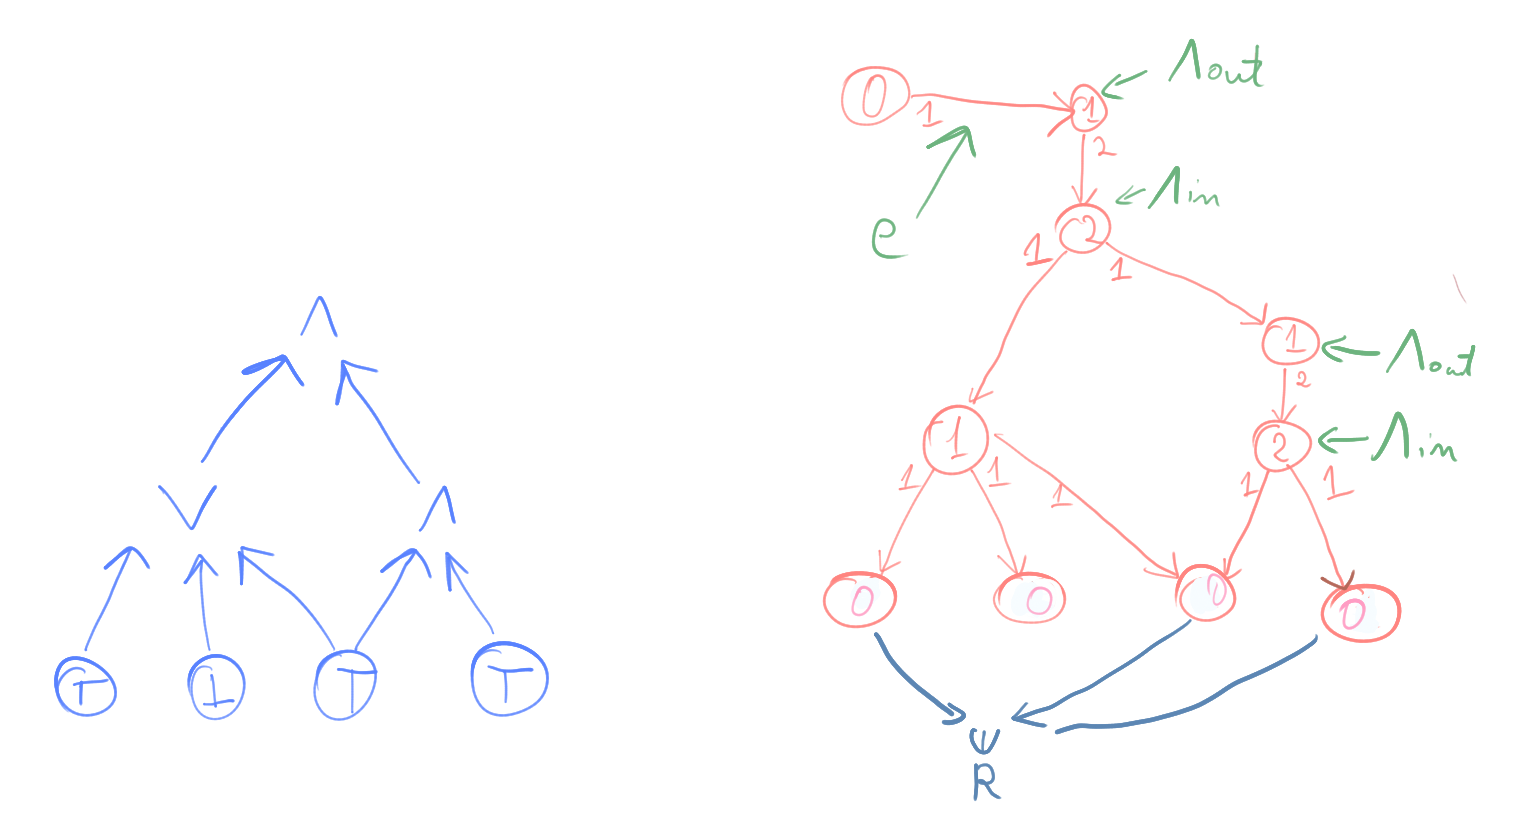
\includegraphics[scale=0.2]{content/graphics/game15.png}
\end{figure}
Note that the edges coming to nodes set to false will never be reversed. True values will propagate
"upwards" the graph.
$e$ will be reversed after some sequence of moves if and only if the circuit evaluates to true.\\

\noindent
\textbf{2. Show that it remains P-complete on planar graphs.}\\
Of course it remains in P on planar graphs, so it suffices to show that it is still P-hard.

\textbf{
      3. Show that it remains P-complete if we restict to graphs whose vertices have
      degrees at most 3 and the possible weights of both vertices and edges are
      \{1, 2\}.
}\\
Here I will use the solution from the first subproblem but add one more assumption: that the provided
boolean circuit for CVP has vertices with degrees at most $2$, and both input degrees and output degrees
are at most 2 for each node.
It is clear that, with such assumption, my reduction to zero-player flow game from the first subproblem
will produce nodes and edges with weights not larger than $2$. The nodes with weight $0$ (input nodes
and the dummy top node) can be handled easily: input nodes' weights can be changed to $1$ without rendering
the graph illegal. For the dummy top node, it is enough to "plug" it to a small cycle with weights $1$.
See the illustration below:
\begin{figure}[H]
      \centering
      \caption{A small modification of the reduction from the first subproblem to get rid of weights equal to $0$.}
      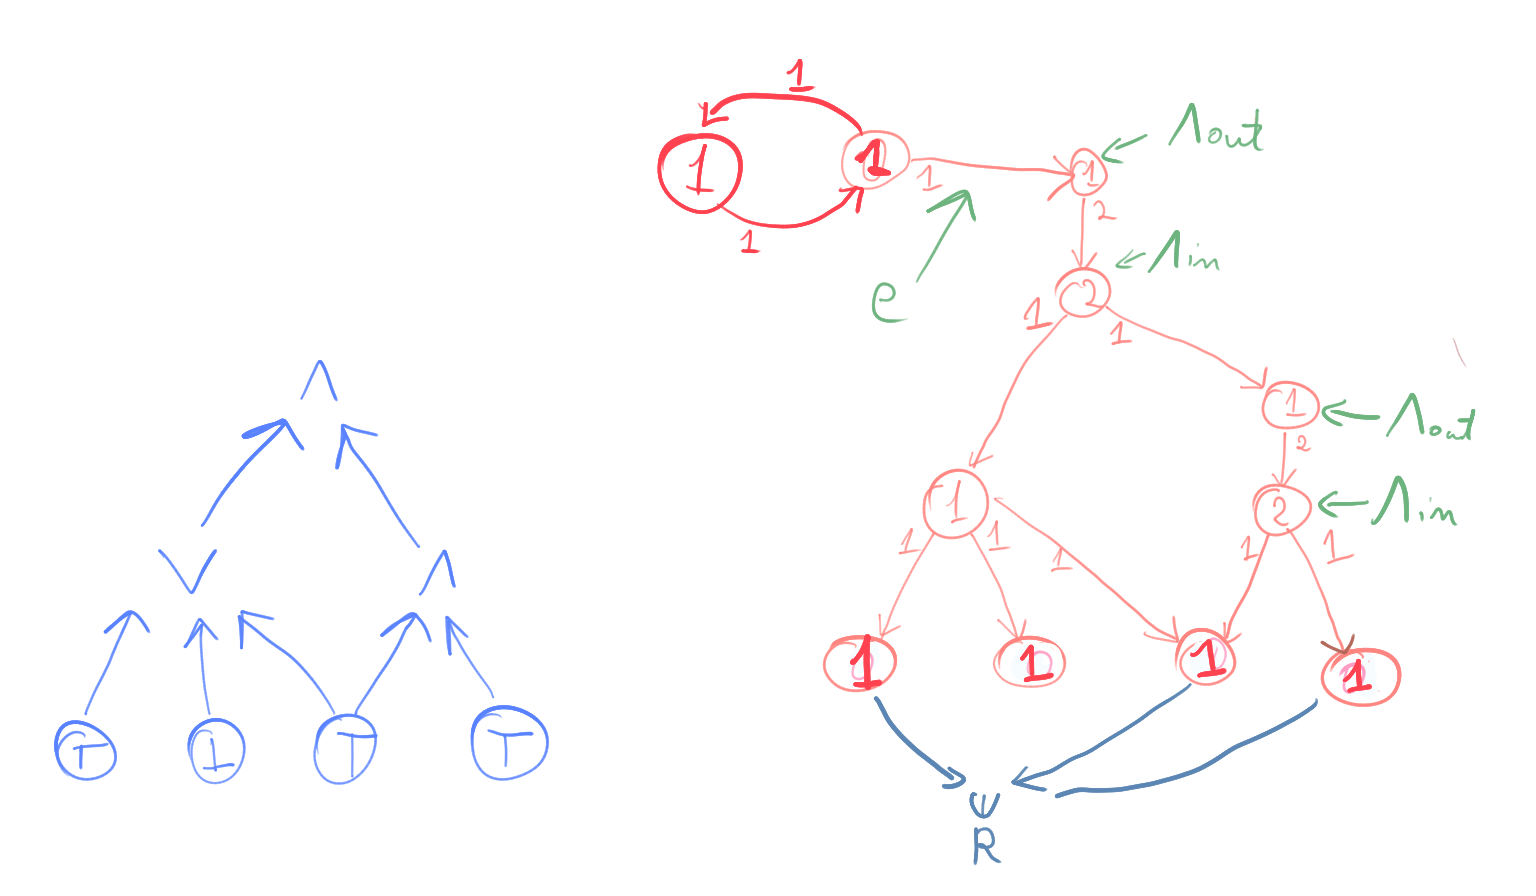
\includegraphics[scale=0.2]{content/graphics/game16.png}
\end{figure}
I have made an assumption that all vertices in the provided circuit have a degree at most 3, and neither input degree
nor output degree is larger than 2 for any node and I will justify that every circuit can be transformed to satisfy this
assumption in reasonable (polynomial) time.

First, every node such that both input and output degree are larger than 1, is split into two, connected by a single edge.
One node handles all input edges, the second -- all output edges. Both nodes perform the same boolean operation as the original
one. This procedure is performed while there is at least one vertex with input and output degree larger than 1.\\
Next, every node with input degree higher than 2 is split into 3 nodes, such that all input edges are divided evenly ($\pm 1$)
between two of them and the third one aggregates their results (refer to the drawing below). This procedure is performed iteratively
while possible.\\
The last step is to perform analogous procedure for outgoing edges. It is also performed iteratively while possible.
\begin{figure}[H]
      \centering
      \caption{
            The three rules to apply iteratively (while possible) to reduce the input and output degrees of
            the nodes in given boolean circuit. For $\lor$ those rules are of course analogous.
      }
      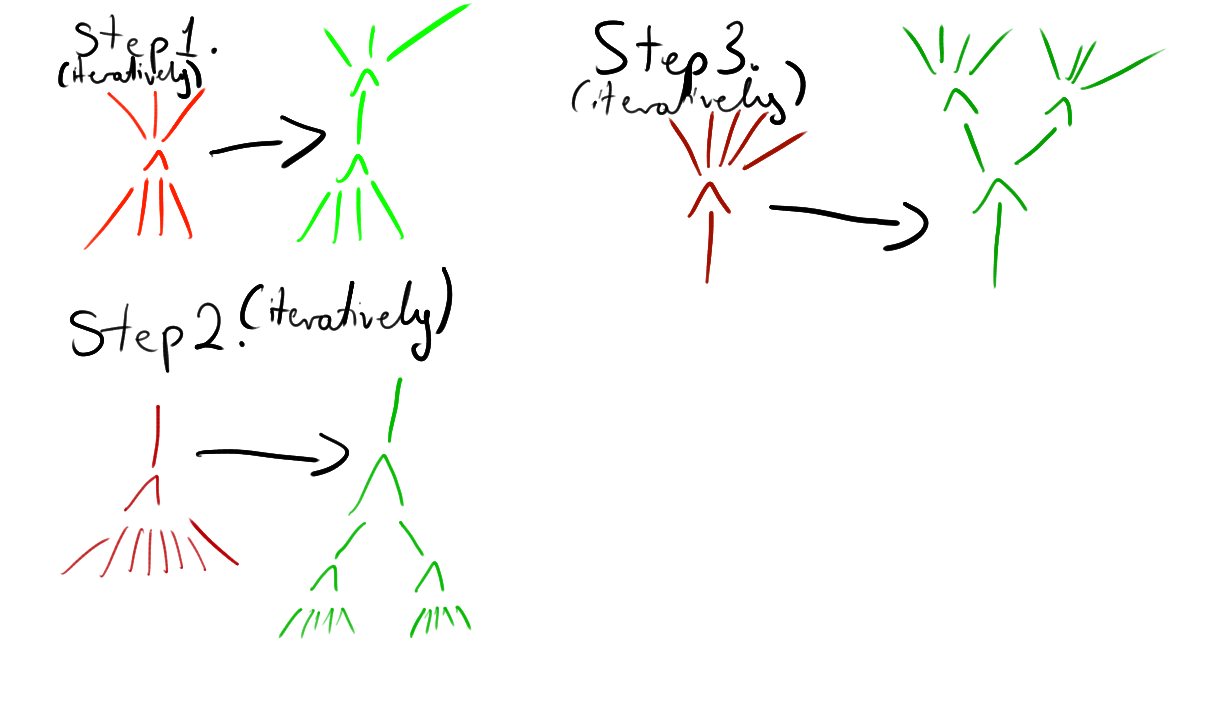
\includegraphics[scale=0.2]{content/graphics/game17.png}
\end{figure}